\section{Leitner's Learning Box reviewed}

% Mention the visual validation tool?
\emph{Leitner's learning box}\footnote{http://en.wikipedia.org/wiki/Leitner\_system} is a simple, but ingenious little contraption to support the tedious
process of memorization, especially prominent when trying to learn, for example, a new language. As depicted in Fig.~\ref{fig:membox_depiction}, this box
consists of a series of partitions with a strict set of rules. The contents to be memorized are written on little cards and placed in the first container. Every
time the user correctly answers a card, that card is promoted to the next partition. Once it reaches the final partition, it can be considered memorized, and
no longer needs to be practiced. Every time the user incorrectly answers a card however, it is sent back to the original starting partition, and the
learning process is restarted.

\begin{figure}[htbp]
	\centering
  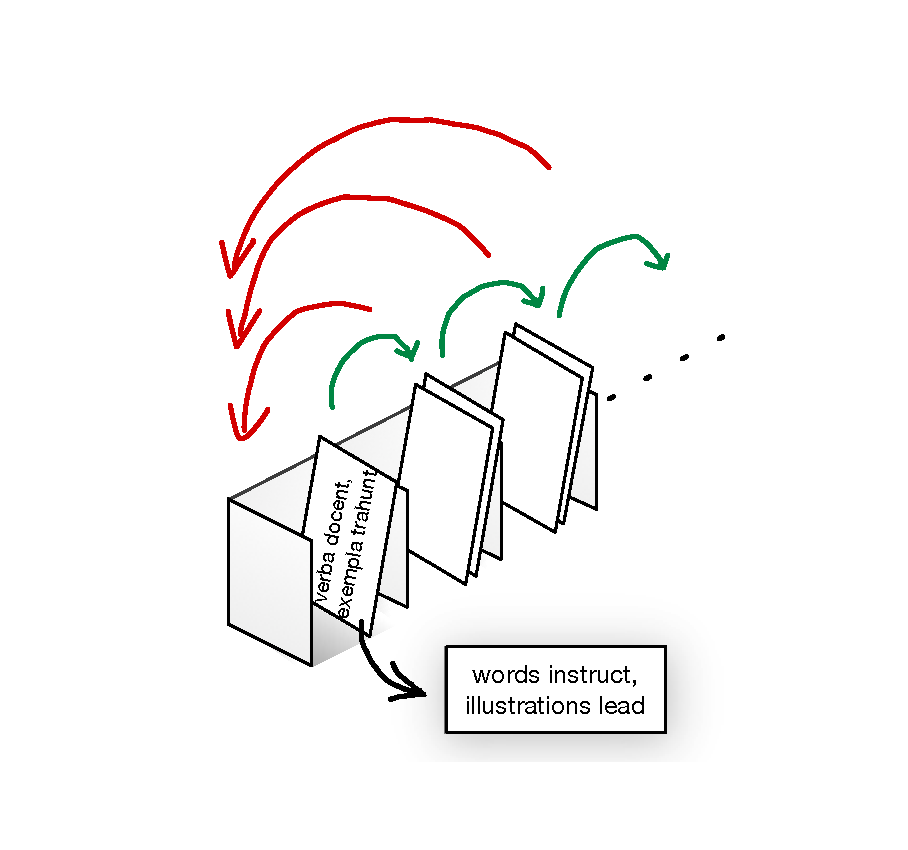
\includegraphics[width=0.4\textwidth]{membox_illustration.pdf}
	\caption{Static Structure of a Leitner's Learning Box}
	\label{fig:membox_depiction}
\end{figure}
\FloatBarrier

For a more detailed overview of the box and our goals, we recommend you read the introduction to Part II. But for now, enough discussion!

\begin{itemize}

\item[$\blacktriangleright$] To get started, press the \texttt{new} button and navigate to ``Examples/eMoflon Handbook Examples/''
(Fig.~\ref{fig:downloadWizard}).

\begin{figure}[htbp]
	\centering
  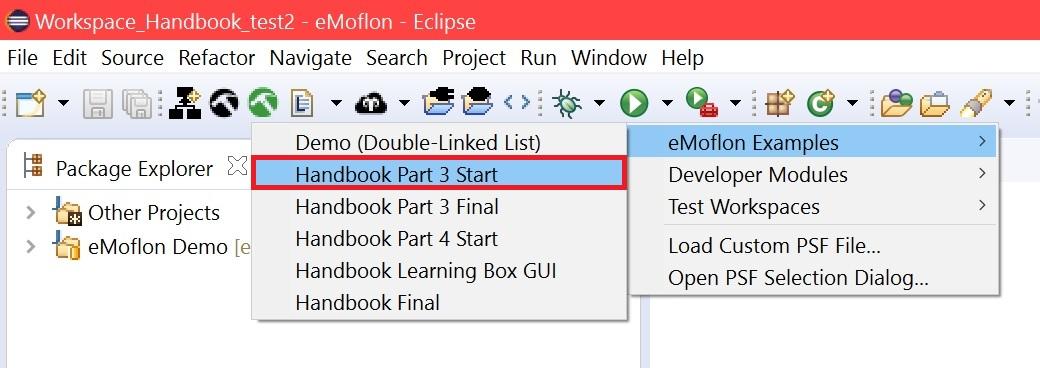
\includegraphics[width=0.65\textwidth]{eclipse_downloadWizard}
	\caption{Download the file set to get started}
	\label{fig:downloadWizard}
\end{figure}
\FloatBarrier

\item[$\blacktriangleright$] Download the file package of the eMolfon syntax type you'd like to learn about. Remember, there's no difference between the
two - this is purely a matter of preference.

\item[$\blacktriangleright$] If your package explorer does not resemble ours in Fig.~\ref{fig:workingSets}, select the small, downward facing arrow in the
corner of the module window. Choose ``Working Sets'' as your top level elements. We work with many working sets, and use them to structure the workspace in 
Eclipse.

\begin{figure}[htbp]
	\centering
  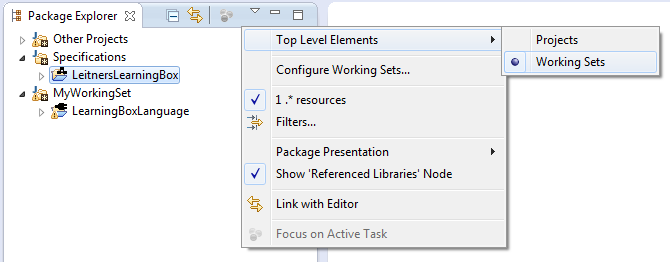
\includegraphics[width=0.9\textwidth]{eclipse_workingSets}
	\caption{Setting your Package Explorer}
	\label{fig:workingSets}
\end{figure}
\FloatBarrier

\fancyfoot[R]{ $\triangleright$ \hyperlink{explanation}{Next Step} }

You should have two nodes, each containing a project file. \texttt{LeitnersLearningBox} contains the metamodel project, which in turn generated the model
instance found in \texttt{LearningBoxLanguage}. They are not contained within the same node as \texttt{LearningBoxLanguage} is a different \emph{nature}, or
project type, than the metamodel project. This is your \emph{repository project}, the Eclipse classification for a normal Java project. For more details on
the project structure, review section 4 of Part I.

\item[$\blacktriangleright$] Inspect the files to get familiar with what you'll be working with. In particular, look at your metamodel structure in the
\texttt{MOSL} folder. You'll be able to see everything defined here also defined in the corresponding \texttt{.ecore} model file in
``LearningBoxLanguage/model/''. We also invite you to browse the files in \texttt{gen}. For details on their contents, refer to Part II, section 5.

\item[$\blacktriangleright$] Well, that's it! A quick review, paired with a fine download makes an excellent appetizer to SDMs. 

\end{itemize}
